\documentclass[border=10pt]{standalone}

\usepackage{tikz}
\usepackage{tikzsymbols}
\usetikzlibrary{calc,patterns,shapes.geometric}

\def\centerarc[#1](#2)(#3:#4:#5){\draw[#1] ($(#2)+({#5*cos(#3)},{#5*sin(#3)})$) arc (#3:#4:#5);}

\begin{document}
	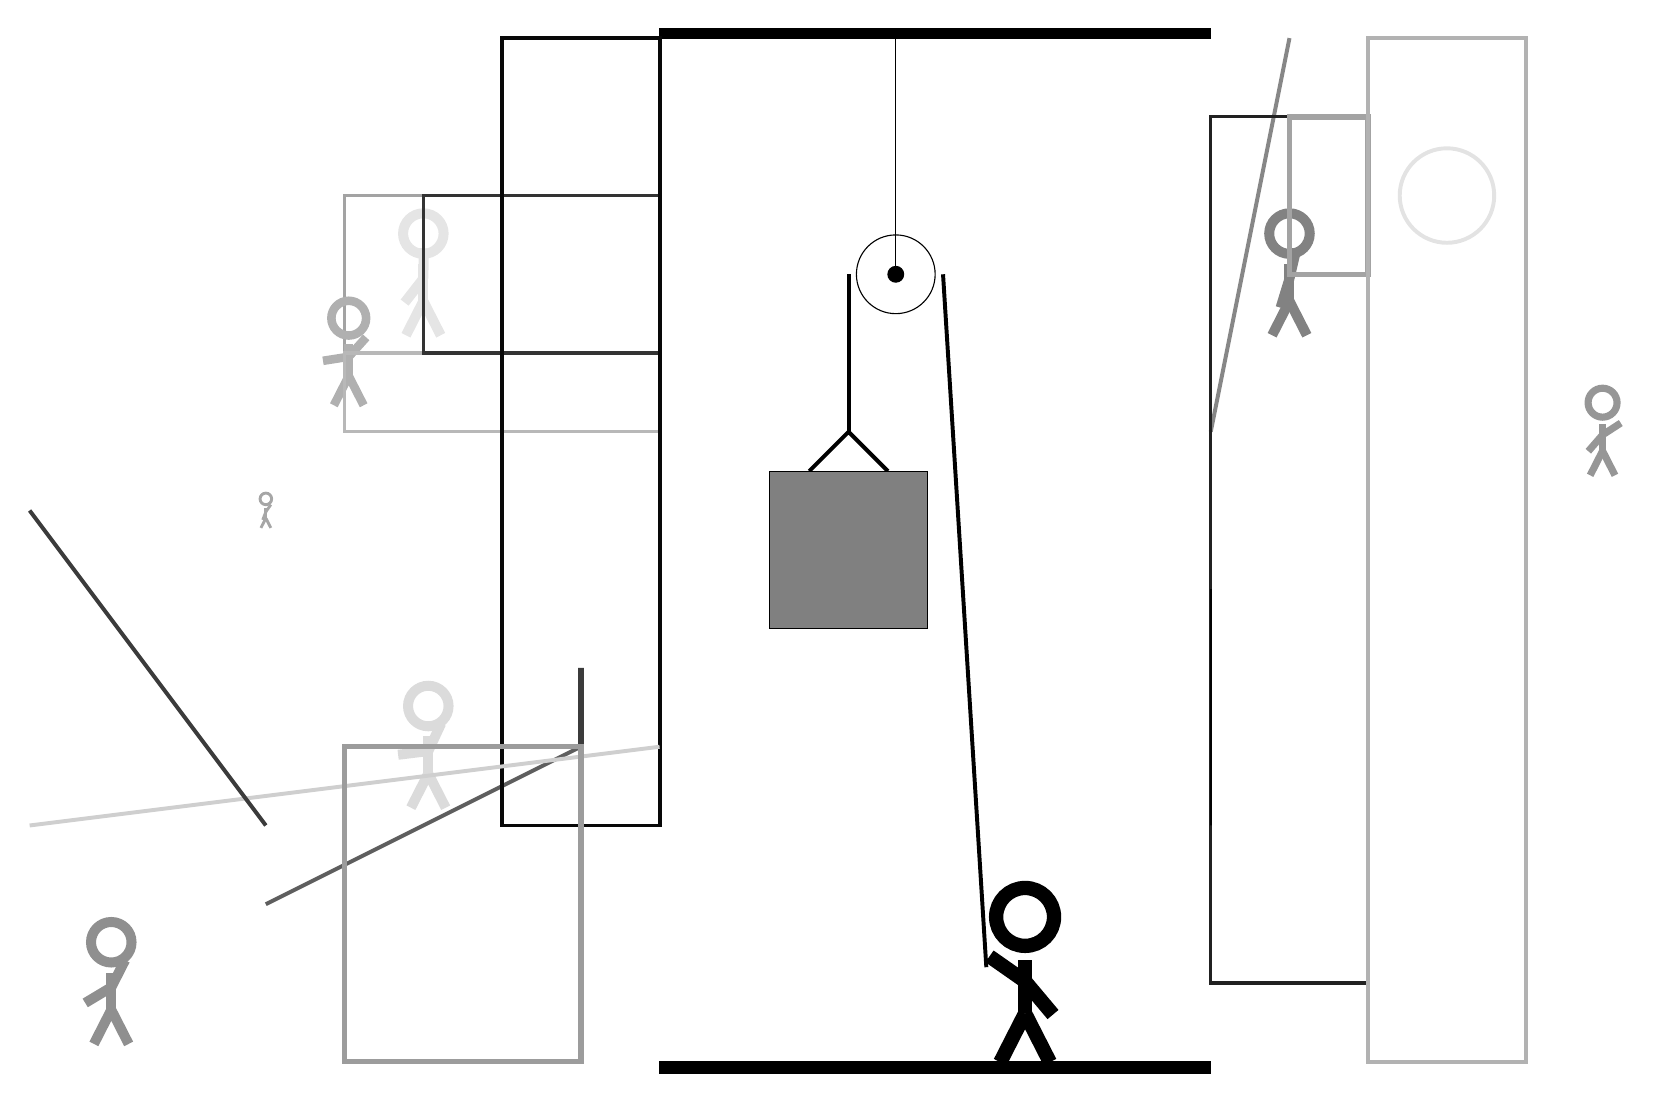
\begin{tikzpicture}
		%%%%% START %%%%%
		
		\draw[fill=black] (-2, 10) rectangle (5, 10.125);
		
		\draw (1, 7) circle (0.5);
		\draw[fill=black] (1, 7) circle (0.1);
		\draw (1, 10) -- (1, 7);
		
		\draw[line width=0.5mm] (-0.1, 4.5) -- (0.4, 5.0) -- (0.9, 4.5);
		\draw[fill=black!50] (-0.6, 4.5) rectangle (1.4, 2.5);
		
		\draw[line width=0.5mm] (0.4, 7) -- (0.4, 5.0);
		\centerarc[line width=0.5mm](1, 7)(0:180:0.6);
		\draw[line width=0.5mm](1.6, 7) -- (2.15, -1.8);
		
		\draw[line width=0.5mm, color=black!63](-3, 1) -- (-7, -1);
		
		\draw[line width=0.4mm, color=black!36] (-4, 5) rectangle (-6, 8);
		\node[line width=0.3mm, color=black!31] at (-6, 6) {\Strichmaxerl[6][9][48]};
		\node[line width=0.7mm, color=black!10] at (-5, 7) {\Strichmaxerl[7][52][89]};
		\node[line width=0.3mm, color=black!14] at (-5, 1) {\Strichmaxerl[7][7][65]};
		
		\draw[line width=0.5mm, color=black!47](6, 10) -- (5, 5);
		
		\draw [line width=0.5mm, color=black!11](8, 8) circle (0.6);
		\node[line width=0.4mm, color=black!44] at (-9, -2) {\Strichmaxerl[7][31][63]};
		\draw[line width=0.7mm, color=black!77] (-3, 2) rectangle (-3, -2);
		\draw[line width=0.4mm, color=black!28] (-2, 6) rectangle (-6, 5);
		
		\draw[line width=0.4mm, color=black!80] (-2, 8) rectangle (-5, 6);
		\draw[line width=0.5mm, color=black!97] (-2, 10) rectangle (-4, 0);
		\node[line width=0.4mm, color=black!41] at (10, 5) {\Strichmaxerl[5][49][33]};
		
		\draw[line width=0.5mm, color=black!19](-2, 1) -- (-10, 0);
		\node[line width=0.5mm, color=black!49] at (6, 7) {\Strichmaxerl[7][73][77]};
		\draw[line width=0.4mm, color=black!87] (7, -2) rectangle (5, 9);
		\draw[line width=0.7mm, color=black!39] (-3, 1) rectangle (-6, -3);
		
		\draw[line width=0.7mm, color=black!36] (7, 7) rectangle (6, 9);
		\draw[line width=0.2mm, color=black!99] (5, 0) rectangle (5, 3);
		
		\node[line width=0.4mm, color=black!35] at (-7, 4) {\Strichmaxerl[2][69][55]};
		\draw[line width=0.5mm, color=black!30] (7, 10) rectangle (9, -3);
		\draw[line width=0.5mm, color=black!77](-7, 0) -- (-10, 4);
		
		\node at (2.6, -1.9) {\Strichmaxerl[10][-35][-50]};
		
		\draw[fill=black] (-2, -3) rectangle (5, -3.15);
		
		%%%%% END %%%%%
	\end{tikzpicture}
\end{document}